\documentclass[11pt]{article}
\usepackage{amsmath,amssymb}
\usepackage{booktabs}
\usepackage{tikz}
\usetikzlibrary{arrows.meta,positioning,calc}
\usepackage[utf8]{inputenc}
\usepackage{hyperref}

\title{\texorpdfstring{$\lambda$tex2web}{latex2web}}
\author{A LaTeX-to-Website tool that converts academic papers, lecture notes and
slides to a folder of docs-style static files.}
\date{}

\begin{document}
\maketitle

\begin{verbatim}
npm install leoldev/latex2web
\end{verbatim}

See some examples here

\begin{description}
  \item[\href{site/ms.html}{Attention Is All You Need}]
    Vaswani \emph{et al.}, NeurIPS 2017.

    Check out $\lambda$tex2web's figure and table derivation capabilities.

  \item[\href{site/src.html}{The entropy formula for the Ricci flow}]
    Perelman, 2002.

    $\lambda$tex2web works on 40+ pages of tensor calculus too, typesetting 57
    math equations cleanly.

  \item[\href{site/dlc-slides-13-2-attention-mechanisms.html}{Attention Mechanisms}]
    Fran\c{c}ois Fleuret's lecture 13.2, from his deep learning course.

    A demo of $\lambda$tex2web's capabilities in transcribing thirty lecture slides
    on attention mechanisms to a website.
\end{description}

\section{How To Run}

Install from GitHub (Node 20+):

\begin{verbatim}
$ npm install leoldev/latex2web
\end{verbatim}

Then you can run:

\begin{verbatim}
$ npx leoldev/latex2web paper.tex -o dist
\end{verbatim}

If you mean to change the source i.e. for your own config:

\begin{verbatim}
$ git clone https://github.com/leoldev/latex2web
$ cd latex2web && npm install
$ node src/cli.js paper.tex -o dist
\end{verbatim}

Then:

\begin{verbatim}
$ latex2web paper.tex -o dist
$ latex2web paper.tex -o dist --theme notes
$ latex2web paper.tex -o dist --config house.json
\end{verbatim}

If you want to know how this website's code works, \texttt{dist} has a copy of
\texttt{index.html} and a file per document with a shared css. The figures are
then in \texttt{assets} and KaTeX in \texttt{vendor}.

\section{What $\lambda$tex2web does}

Or really, what it can do.

\begin{tabular}{@{}p{0.24\linewidth}p{0.7\linewidth}@{}}
\toprule
\textbf{In LaTeX:} & \textbf{$\lambda$tex2web Out:} \\
\midrule
\texttt{\textbackslash input}, \texttt{\textbackslash include} &
  all included; including nested, section/equation numbers and label scopes \\
\texttt{equation}, \texttt{align}, \texttt{gather}, \texttt{multline},
  \texttt{cases} &
  all math is rendered, including references between equations. \\
\texttt{figure}, \texttt{table}, \texttt{tabular} &
  rendered and captioned (*image files are copied out of the source tree) \\
\texttt{tikzpicture} &
  uses a TeX engine with your preamble's own macros and styles (or shown as
  source) \\
\texttt{lstlisting}, \texttt{verbatim}, \texttt{minted} &
  recognises language syntax and formats code \\
\texttt{thebibliography}, a \texttt{.bbl}, a \texttt{.bib} &
  citations numbered and linked (when possible) \\
\texttt{\textbackslash ref}, \texttt{\textbackslash eqref},
  \texttt{\textbackslash cite} &
  included \\
\texttt{\textbackslash href}, \texttt{\textbackslash url},
  \texttt{\textbackslash footnote} &
  all transcribed as written \\
\bottomrule
\end{tabular}

\section{What it can't do}

$\lambda$tex2web isn't a TeX engine and doesn't plan on being one. There is
unfortunately then no typesetting, no package resolution, and no expansions beyond
\texttt{\textbackslash newcommand} and \texttt{\textbackslash def} in your own
preamble. Anything it doesn't recognised will be spit out as text.

Also:

\begin{itemize}
  \item \textbf{TikZ needs an engine.} Diagrams are compiled with
    \texttt{pdflatex} when installed, so a figure looks like the source. With no
    engine on the machine they appear as source.
  \item \textbf{Vector figures are rasterised.} A PDF inside an \texttt{img}
    element will show nothing, and is why the Ricci flow page is megabytes large.
\end{itemize}

\begin{figure}[h]
\centering
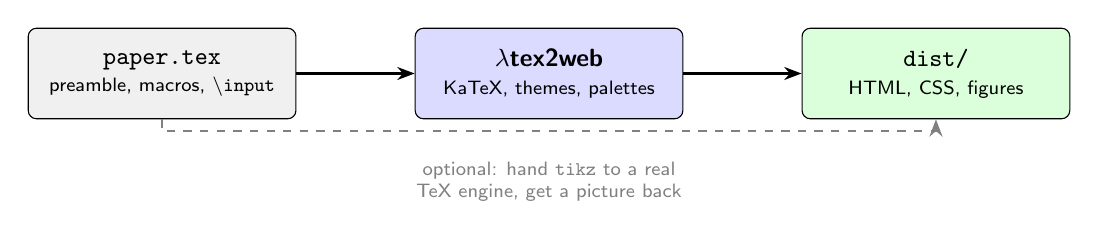
\begin{tikzpicture}[
  font=\sffamily\small,
  box/.style={draw, rounded corners=3pt, minimum width=3.4cm, minimum height=1.15cm,
              align=center, inner sep=4pt},
  flow/.style={-{Stealth[length=2.2mm]}, thick}
]
  \node[box, fill=gray!12] (src) { \texttt{paper.tex}\\[-1pt]
    \scriptsize preamble, macros, \texttt{\textbackslash input} };
  \node[box, fill=blue!14, right=1.5cm of src] (l2w)
    { \textbf{$\lambda$tex2web}\\[-1pt] \scriptsize KaTeX, themes, palettes };
  \node[box, fill=green!14, right=1.5cm of l2w] (out)
    { \texttt{dist/}\\[-1pt] \scriptsize HTML, CSS, figures };
  \draw[flow] (src) -- (l2w);
  \draw[flow] (l2w) -- (out);
  \node[below=0.42cm of l2w, align=center, font=\scriptsize\sffamily, text=gray]
    { optional: hand \texttt{tikz} to a real\\ TeX engine, get a picture back };
  \draw[flow, dashed, gray] (src.south) |- ($(out.south)+(0,-0.15)$) -- (out.south);
\end{tikzpicture}
\caption{Figure 1: What $\lambda$tex2web does by itself. You need a TeX engine to
compile TikZ diagrams.e}
\end{figure}

All three examples featured on this cite went through the same command that built
this page (though with different configurations), from the original LaTeX files
off arxiv. Please refer to the
\href{site/docs.html}{documentation page} for more information.

\end{document}